\begin{frame}{Introducción}
\justifying
Con JavaScript, puede hacer que sus páginas web cobren vida haciendo que interactúen con el usuario. JavaScript es un lenguaje de programación completo y, como tal, todo es posible. 
{\tiny Web Programming with html5, css, and javascript de John Dean (2019)}
\end{frame}

\begin{frame}{Historia de JavaScript 01/04}
\justifying
La primera versión de HTML, diseñada por Tim Berners-Lee de 1989 a 1991, era de naturaleza bastante estática.
Excepto por los saltos de enlace con el elemento a, las páginas web simplemente mostraban contenido, y el contenido se corrigió. En 1995, el fabricante dominante de navegadores era Netscape, y uno de sus empleados, Brendan Eich, pensó que sería útil agregar funcionalidad dinámica a las páginas web. Así que diseñó el lenguaje de programación JavaScript, que agrega funcionalidad dinámica a las páginas web cuando se usa junto con HTML. Por ejemplo, JavaScript proporciona la capacidad de actualizar el contenido de una página web cuando ocurre un evento, como cuando un usuario hace clic en un botón. También proporciona la capacidad de recuperar la entrada de un usuario y procesar esa entrada.
{\tiny Web Programming with html5, css, and javascript de John Dean (2019)}
\end{frame}

\begin{frame}{Historia de JavaScript 02/04}
\justifying
Eich tardó solo 10 días en mayo de 1995 en implementar el lenguaje de programación JavaScript, una hazaña realmente notable. Marc Andreessen, uno de los fundadores de Netscape, originalmente nombró el nuevo lenguaje Mocha y luego LiveScript. Pero para fines de marketing, Andreessen realmente quería el nombre JavaScript. En ese momento, la industria del software estaba entusiasmada con el nuevo lenguaje de programación, Java. Andreessen pensó que todos los devotos del carro de Java gravitarían a su nuevo lenguaje de programación de navegador si tuviera el nombre Java. En diciembre de 1995, Andreessen consiguió su deseo cuando Netscape obtuvo una licencia de marca registrada del fabricante de Java, Sun Microsystems, y el nombre de LiveScript se cambió a JavaScript. Desafortunadamente, muchas, muchas personas a lo largo de los años han cometido el error de suponer que JavaScript es igual a Java o muy cercano a él. No se deje engañar por el nombre: JavaScript no es tan similar a Java. En realidad, C ++ y otros lenguajes de programación populares están más cerca de Java que JavaScript.
{\tiny Web Programming with html5, css, and javascript de John Dean (2019)}
\end{frame}

\begin{frame}{Historia de JavaScript 03/04}
\justifying
En 1996, Netscape envió JavaScript a la organización de estándares Ecma International para promover la influencia de JavaScript en todos los navegadores (no solo en el navegador de Netscape). Ecma International utilizó JavaScript como base para crear el estándar ECMAScript. Como se esperaba, ECMAScript ahora sirve como el estándar para los lenguajes de programación interactivos integrados en todos los navegadores populares de hoy. En el momento de la impresión de este libro, la versión más reciente de ECMAScript es la versión 7, publicada en 2016. Encontrar el nombre de ECMAScript fue un proceso difícil, con diferentes fabricantes de navegadores que tenían opiniones muy opuestas. El creador de JavaScript, Brendan Eich, ha declarado que el resultado, ECMAScript, es "un nombre comercial no deseado que suena como una enfermedad de la piel".
{\tiny Web Programming with html5, css, and javascript de John Dean (2019)}
\end{frame}

\begin{frame}{Historia de JavaScript 04/04}
\justifying
En 1998, Netscape formó la comunidad de software libre Mozilla, que finalmente implementó Firefox, uno de los principales navegadores de hoy. Brendan Eich se mudó a Mozilla, donde él y otros continuaron actualizando JavaScript a lo largo de los años, siguiendo el estándar ECMAScript establecido por Ecma International.

Otros fabricantes de navegadores admiten sus propias versiones de JavaScript. Para sus navegadores Internet Explorer y Edge, Microsoft usa JScript. Para su navegador Chrome, Google usa el motor V8 JavaScript. Afortunadamente, todos los fabricantes de navegadores intentan seguir el estándar ECMAScript, por lo que para la mayoría de las tareas, los programadores pueden escribir una versión de su código y funcionará para todos los navegadores diferentes. En este libro, nos atenemos al código ECMAScript estándar que funciona igual en todos los navegadores. Como con casi todos en la comunidad de programación web, nos referimos a nuestro código como JavaScript, a pesar de que JavaScript es solo una de varias implementaciones de ECMAScript (JavaScript es la implementación utilizada en Firefox de Mozilla).
{\tiny Web Programming with html5, css, and javascript de John Dean (2019)}
\end{frame}

\begin{frame}{Hola mundo en mi primera página web 01/02}
\justifying
\begin{figure}[H]
\centering
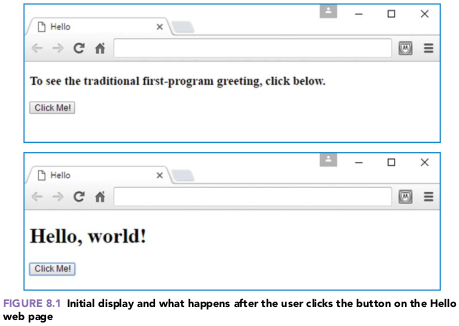
\includegraphics[scale=0.5]{Section_Files/images/Sec01/01.png}
\caption{Pantalla del 'hola mundo'.}
\end{figure}

{\tiny Web Programming with html5, css, and javascript de John Dean (2019)}
\end{frame}

\begin{frame}{Hola mundo en mi primera página web 02/02}
\justifying
\begin{figure}[H]
\centering
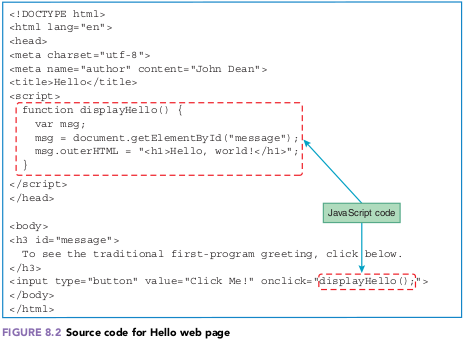
\includegraphics[scale=0.5]{Section_Files/images/Sec01/02.png}
\caption{Código del 'hola mundo'.}
\end{figure}

{\tiny Web Programming with html5, css, and javascript de John Dean (2019)}
\end{frame}

\begin{frame}{Botones 01/03}
\justifying
Existen diferentes tipos de botones, cada uno con su propia sintaxis. Para simplificar las cosas, comenzaremos con un solo tipo de botón, y aquí está su sintaxis:
\begin{figure}[H]
\centering
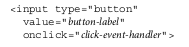
\includegraphics[scale=0.5]{Section_Files/images/Sec01/03.png}
\caption{Sintáxis.}
Tenga en cuenta que el código es un elemento vacío que utiliza la etiqueta de entrada. Como su nombre lo indica, la etiqueta de entrada implementa elementos que manejan la entrada del usuario. Es posible que no piense en un botón como una entrada del usuario, pero lo es: el usuario elige hacer algo haciendo clic en un botón. Más adelante, presentaremos otros elementos de entrada del usuario (por ejemplo, controles de texto y casillas de verificación) que también usan la etiqueta de entrada.
\end{figure}

\end{frame}

\begin{frame}{Botones 02/03}
\justifying
Como lo hemos hecho a lo largo del libro al introducir nuevas construcciones, el fragmento de código anterior muestra solo los detalles de sintaxis más importantes, para que no se sienta abrumado con demasiado para recordar. Mostramos los atributos más comunes del elemento de entrada: tipo, valor y onclick. Observe cómo el elemento de entrada en la parte inferior de la Figura 8.2 sigue este patrón de sintaxis e incluye esos tres atributos.

El elemento de entrada se usa para diferentes tipos de entrada de usuario, y su atributo de tipo especifica qué tipo de entrada de usuario. Más formalmente, el atributo type especifica el tipo de control que se está implementando, donde un control es una entidad de entrada del usuario, como un botón, control de texto o casilla de verificación. En el código fuente de la página web Hello, tenga en cuenta que el atributo type obtiene el botón de valor, que le indica al navegador que muestre un botón. Si no proporciona un atributo de tipo, el navegador mostrará un control de texto, porque ese es el tipo de control predeterminado para el elemento de entrada. Describiremos los controles de texto más adelante en este capítulo. Por ahora, solo sepa que un control de texto es un cuadro en el que un usuario puede ingresar texto, y así es como se ve un control de texto (completado) (con un mensaje a su izquierda):


{\tiny Web Programming with html5, css, and javascript de John Dean (2019)}
\end{frame}

\begin{frame}{Botones 03/03}
\justifying
\begin{figure}[H]
\centering

\includegraphics[scale=0.5]{Section_Files/images/Sec01/04.png}
\caption{El usuario puede ingresar texto.}
\end{figure}
Debido a que utiliza un cuadro, muchos desarrolladores web se refieren a los controles de texto como "cuadros de texto". Usamos el término "control de texto" porque es el término utilizado con mayor frecuencia por las organizaciones de estándares HTML.
El atributo de valor del elemento de entrada especifica la etiqueta del botón. Si no proporciona un atributo de valor, el botón no tendrá etiqueta. Si desea un botón sin etiqueta, en lugar de simplemente omitir el atributo de valor, le recomendamos que especifique value = "". Esa es una forma de autodocumentación y hace que su código sea más comprensible.


{\tiny Web Programming with html5, css, and javascript de John Dean (2019)}
\end{frame}
